
%(BEGIN_QUESTION)
% Copyright 2010, Tony R. Kuphaldt, released under the Creative Commons Attribution License (v 1.0)
% This means you may do almost anything with this work of mine, so long as you give me proper credit

Determine the process conditions (temperature and flow rate) sensed by the switches, given their trip settings and the voltage measurement shown.  Assume the circuit is functioning properly and has no faults, electrical or otherwise:

$$\includegraphics[width=15.5cm]{i01897x01.eps}$$

Of course, you will not be able to determine {\it precise} process values, but you should be able to determine whether a variable is above or below a certain value.  If the voltage measurement cannot prove the process condition one way or another, write ``inconclusive'' for your answer.

\vskip 30pt

Process temperature = 

\vskip 30pt

Process flow rate = 

\underbar{file i01897}
%(END_QUESTION)





%(BEGIN_ANSWER)

Process temperature = {\bf more than 150 $^{o}$F}

Process flow rate = {\bf less than 9.2 GPM}

%(END_ANSWER)





%(BEGIN_NOTES)

{\bf This question is intended for exams only and not worksheets!}.

%(END_NOTES)

